\documentclass[border=3pt]{standalone}
% Shared preamble for every generated figure.
% Matches the report: newtx (Times), greyscale, square boxes.
\usepackage{newtxtext,newtxmath}
% newtx's typewriter (txtt) draws a slashed zero; use Latin Modern instead.
\renewcommand{\ttdefault}{lmtt}
\usepackage{tikz}
\usetikzlibrary{positioning,arrows.meta,calc,fit,backgrounds,shapes.geometric,
                decorations.pathreplacing,decorations.pathmorphing,matrix,patterns}

\definecolor{figgrey}{gray}{0.88}
\definecolor{figmid}{gray}{0.60}
\definecolor{figdark}{gray}{0.35}

\tikzset{
  fig/.style={font=\small},
  box/.style={draw,thick,minimum height=8mm,minimum width=22mm,align=center,
              inner sep=2pt,font=\small},
  greybox/.style={box,fill=figgrey},
  smallbox/.style={draw,minimum height=6mm,minimum width=16mm,align=center,
                   inner sep=2pt,font=\scriptsize},
  ln/.style={-{Stealth[length=2.2mm,width=1.8mm]},thick},
  lnb/.style={{Stealth[length=2.2mm,width=1.8mm]}-{Stealth[length=2.2mm,width=1.8mm]},thick},
  lbl/.style={font=\scriptsize,inner sep=1.5pt},
  note/.style={font=\scriptsize\itshape,inner sep=1.5pt},
}

\begin{document}
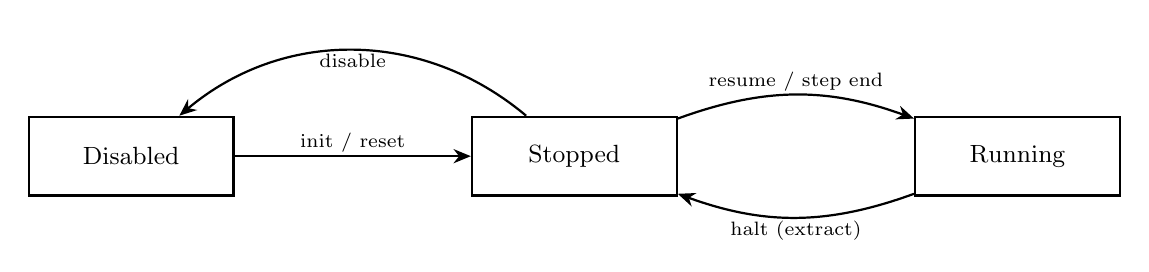
\begin{tikzpicture}[fig,
  st/.style={draw,thick,minimum height=10mm,minimum width=26mm,align=center,font=\small},
  ev/.style={font=\scriptsize,align=center,inner sep=1pt}]

\node[st] (dis) {Disabled};
\node[st,right=30mm of dis] (stp) {Stopped};
\node[st,right=30mm of stp] (run) {Running};

\draw[ln] (dis) -- node[ev,above]{init / reset} (stp);
\draw[ln] (stp) to[bend left=20] node[ev,above]{resume / step end} (run);
\draw[ln] (run) to[bend left=20] node[ev,below]{halt (extract)} (stp);
\draw[ln] (stp) to[bend right=40] node[ev,below]{disable} (dis);

\end{tikzpicture}
\end{document}
